\documentclass[12pt,a4paper]{article}
\usepackage[margin=1in]{geometry}
\usepackage{amsmath}
\usepackage{graphicx}
\usepackage{hyperref}
\usepackage[authoryear]{natbib}
\usepackage{xcolor}
\usepackage{setspace}
\usepackage{float}

\definecolor{brandblue}{HTML}{00466F}
\definecolor{brandorange}{HTML}{F38C10}
\definecolor{brandteal}{HTML}{037E73}
\definecolor{brandgray}{HTML}{3D3D3D}
\hypersetup{colorlinks=true, linkcolor=brandblue, citecolor=brandteal, urlcolor=brandblue}
\onehalfspacing

\title{Monthly USD/CHF Covered Interest Parity Deviations}
\author{Iv\'an Weigandi}
\date{\today}

\begin{document}
\maketitle

\begin{abstract}
\noindent This note describes the construction of monthly covered interest parity (CIP) deviation measures for the USD/CHF pair. The series combine spot and forward exchange rates with short-term USD and CHF interest-rate benchmarks. The resulting measures distinguish between risk-free-rate benchmarks based on SOFR and SARON, legacy LIBOR benchmarks, and government money-market rate proxies.
\end{abstract}

\section{Definition}

Let \(S_t\) denote the spot exchange rate quoted in CHF per USD, and let \(F_t^{(T)}\) denote the corresponding forward exchange rate for tenor \(T\). With this quote convention, the forward-implied USD minus CHF interest-rate differential is
\begin{equation}
    \widehat{r}_{USD,t}^{(T)} - \widehat{r}_{CHF,t}^{(T)} = -\frac{1}{T}\log\left(\frac{F_t^{(T)}}{S_t}\right).
\end{equation}

The CIP deviation is defined as the difference between the observed interest-rate differential and the forward-implied differential:
\begin{equation}
    b_t^{(T)} = \left(r_{USD,t}^{(T)} - r_{CHF,t}^{(T)}\right)
    - \left[-\frac{1}{T}\log\left(\frac{F_t^{(T)}}{S_t}\right)\right].
\end{equation}
The published series report \(10000 \times b_t^{(T)}\), so values are annualized basis points.

\section{Data}

The exchange-rate data are from the Swiss National Bank and include USD/CHF spot, three-month forward, and six-month forward rates. The modern risk-free-rate measures use SOFR from FRED and SARON compound rates from the Swiss National Bank. The legacy measure uses USD and CHF LIBOR series. A government-rate proxy combines the US Treasury bill rate from FRED with the Swiss Confederation money-market series from the Swiss National Bank.

\section{Series}

The public dataset contains four main basis measures: three-month SOFR-SARON, six-month SOFR-SARON, three-month LIBOR, and a three-month government-rate proxy. These are related but distinct measures and should not be treated as interchangeable. They reflect different benchmark markets and, for the legacy LIBOR series, a different institutional environment.

\section{Chart}

Figure~\ref{fig:cip} plots the monthly basis measures in basis points.

\begin{figure}[H]
    \centering
    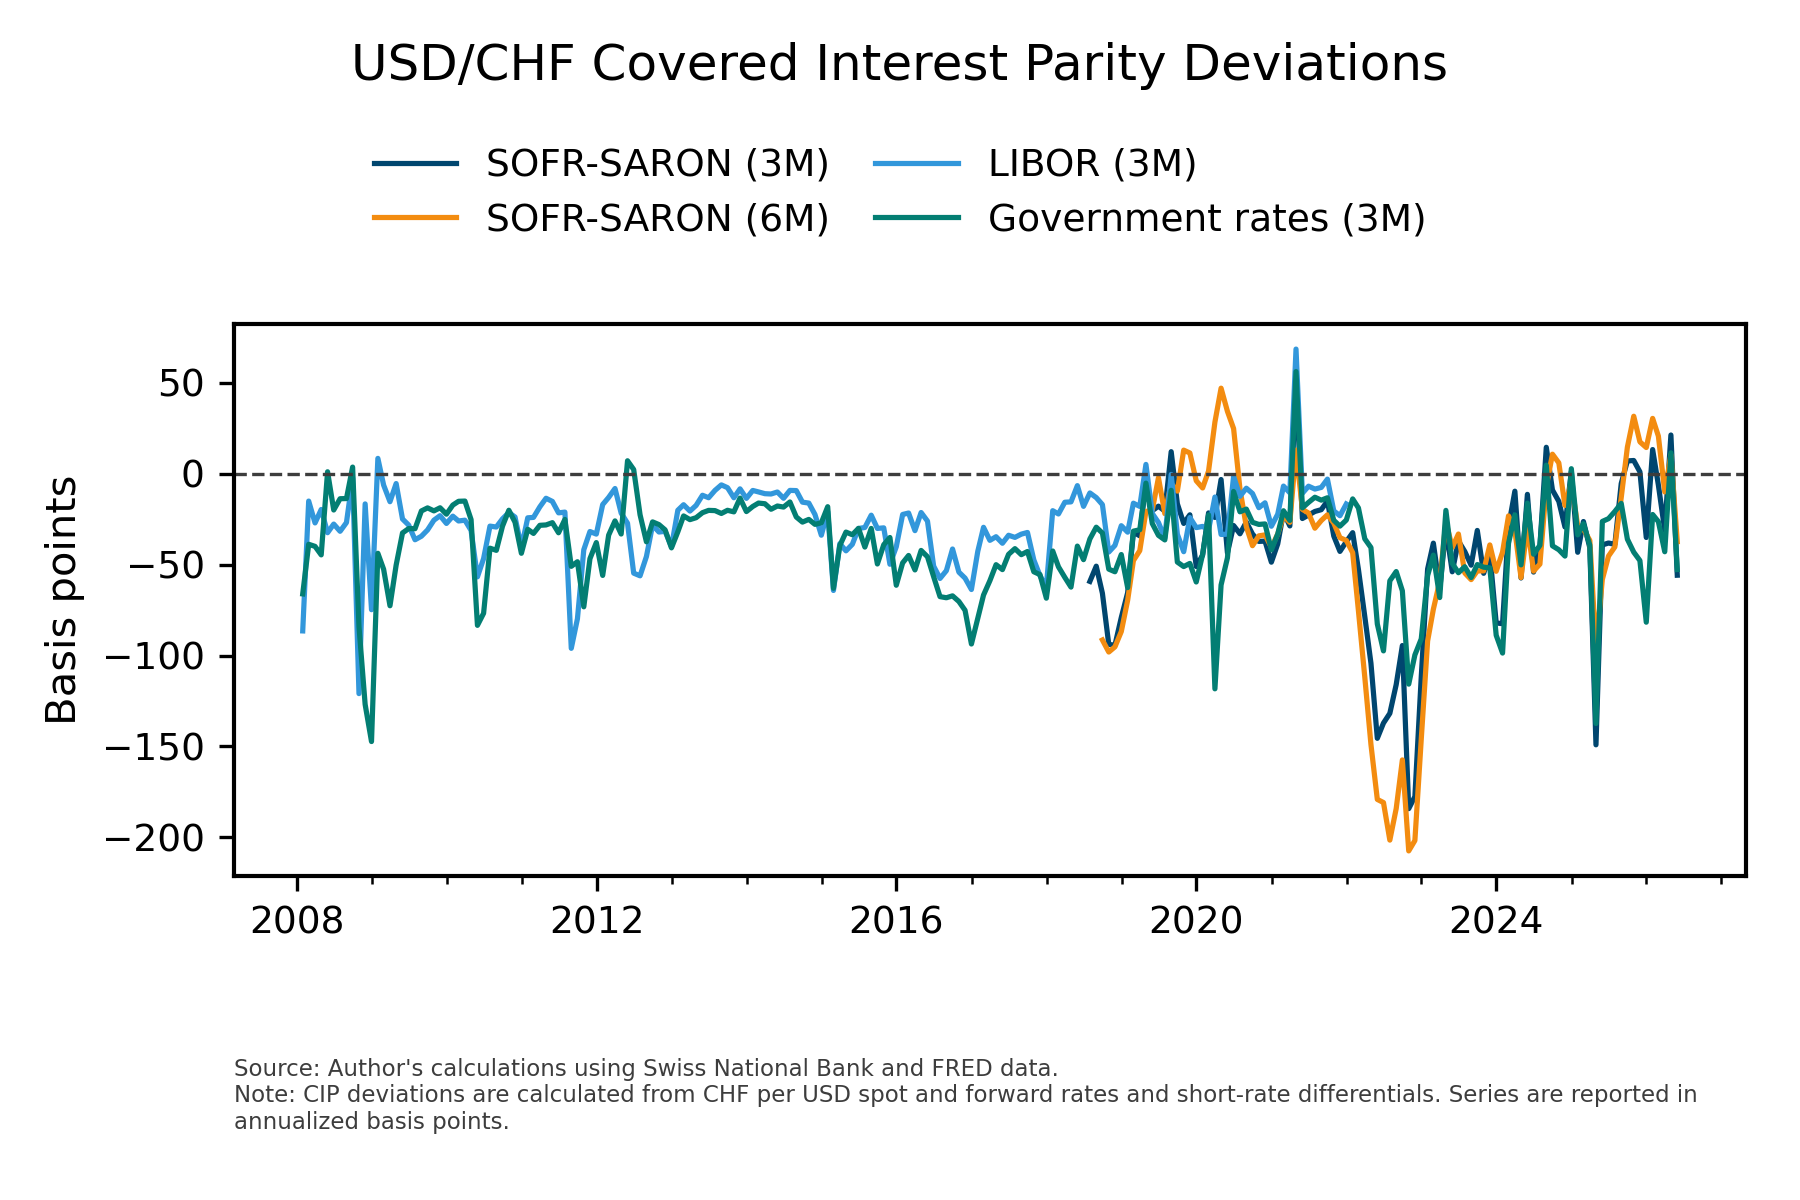
\includegraphics[width=\linewidth]{../chart/usd_chf_cip_deviations.png}
    \caption{Monthly USD/CHF covered interest parity deviations}
    \label{fig:cip}
\end{figure}

\section{Replication}

The replication script downloads public data from the Swiss National Bank and FRED, computes the series, writes source diagnostics, and regenerates the chart. Source diagnostics are included to make the sample coverage of each input series transparent.

\begin{thebibliography}{9}
\bibitem[Miranda-Agrippino and Rey(2020)]{MirandaRey2020}
Miranda-Agrippino, S., \& Rey, H. (2020). US monetary policy and the global financial cycle. \textit{The Review of Economic Studies}, 87(6), 2754--2776.
\end{thebibliography}

\end{document}
